%%%%%%
% OS %
%%%%%%

\section{Struktura OS – systémové jádro, monolitický systém, architektura klient-server, virtuální stroje} \label{kernel}

Operační systém si lze (opravdu zjednodušeně) představit jako program skládající se z \textit{jádra} (tj. \textit{kernel}) a \textit{systémových programů}. \textit{Systémové programy} jsou takové programy, které poskytují prostředí pro spouštění a běh \textit{aplikačních programů} (aplikace které nejsou součástí OS). Dále pak  \textit{systémová volání} fungují jako jakési API pro \textit{systémové programy} aby mohly volat funkce z jádra. (toto např. umožňuje čtení\footnote{pomocí systémového volání \textit{open}, kde můžeme nastavovat různé možnosti, jako \textit{O\_APPEND,O\_CREAT}} ze souboru nebo jejich vytváření\footnote{může se například vytvořit pomocí systémového volání \textit{open} s možností \textit{O\_CREAT}, která soubor vytvoří pokud neexistuje})

\begin{enumerate}
    \item Systémové programy -- knihovny
    \item Aplikační programy -- prohlížeč, textový editor, apod. 
\end{enumerate}
    
\begin{center}
    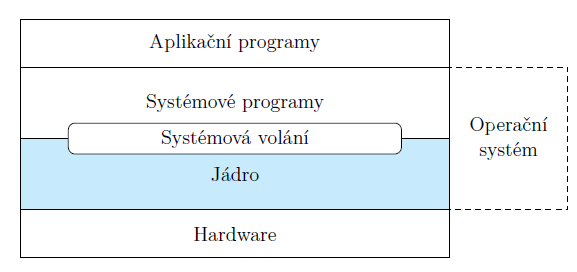
\includegraphics[scale=1]{images/OS_kernel_apps.png}
\end{center}

V Operačních Systémech zpravidla rozlišujeme dva základní režimy operací:

\begin{enumerate}
    \item režim jádra tj. privilegovaný/systémový režim
    \item uživatelský režim tj. neprivilegovaný režim
\end{enumerate}

V uživatelském režimu běží všechny aplikace, krom jádra. Více viz \ref{procesy}.

\begin{Large}
    \vspace{0,5cm} 
    \textbf{Monolitický systém}\\
\end{Large}

Jak již napovídá samotný název, \textit{monolitický systém} je systém který prakticky nemá skoro žádnou strukturu. Jádro je pouze souhrn procedur, které se navzájem volají. Tento druh jádra vzniká kompilací zdrojových kódů na objektové soubory (končící na .o), tyto objektové soubory jsou potom \textit{svázány}/\textit{spojeny} v tzv. \textit{linkeru} do jednoho spustitelného souboru. Tady vyplývá na povrch první značná nevýhoda \textit{monolitických} jader, při jakékoliv změně v jádře je třeba jej kompletně překompilovat! 

\begin{center}
    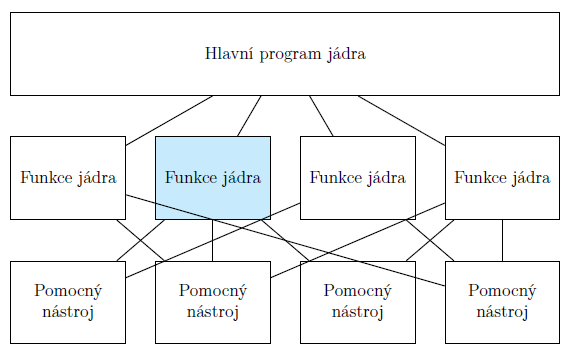
\includegraphics[scale=1]{images/OS_mono_kernel.png}
\end{center}

I když jsme si řekli, že tento systém vlastně žádnou strukturu nemá, šla by i tak popsat takto (s pomocí obrázku výše):

\begin{itemize}
    \item Hlavní program volající vyžádanou funkci
    \item Množina funkcí obsluhující systémová volání
    \item Sada nástrojů, které pomáhají funkcím
\end{itemize}

Hlavní jádro spouští funkce potřebné pro obsloužení systémových volání/přerušení (každé volání/přerušení obsluhuje jedna funkce). Pomocné nástroje pak provádí akce vyžádané funkcemi. 

\begin{large}
    \vspace{0,5cm}
    \textbf{Problémy s monolitickým jádrem a jejich řešení}\\
\end{large}

I když je monolitická architektura rychlá, má jednu značnou nevýhodu. Jedna chyba v jádře (anpř. v ovladači) může shodit celý systém. Jádro je sice od uživatelských aplikací odděleno pomocí systémových volání, a tedy chráněno před zastavením chybou v uživatelských aplikacích, ale před problémem v ovladači, jádře nebo jiných systémových službách už nikoliv.\\

Možným řešením je tzv. \textbf{modulární jádro}. Jádro jako takové obsahuje pouze části nutné pro běh, ostatní části (tzv. \textit{moduly}) jsou dynamicky načítány podle potřeby. Načítat se může při startu systému nebo i během činnosti. Výhody tohoto sytému:

\begin{itemize}
    \item Po aktualizaci/změně modulů není třeba znovu kompilovat jádro
    \item Menší velikost jádra
\end{itemize}

Moduly bývají ovladače zařízení a souborových systémů. Chyba v modulu může zastavit proces (pokud běží v procesovém kontextu v rámci obsluhy sys. volání) nebo celý systém (pokud obsluhuje sys. přerušení).

\newpage

\begin{Large}
    \vspace{0,5cm} 
    \textbf{Systém klient-server}\\
\end{Large}

Tento systém opět zmenšuje kernel až na tzv. \textit{mikrojádro}. V něm zůstanou pouze nezbytné funkce jako správa paměti, multitasking, přerušení a komunikace mezi procesy. Vše ostatní je přesunuto do tzv. \textit{serverů} což je software běžící v uživatelském režimu. Žádost o sys. volání tedy znamená, že aplikace (klient) zašle žádost \textit{serveru} kde jádro mezi nimi zprostředkovává komunikaci. \\

Z tohoto vyplývá, že chyba v \textit{serveru} nebude fatální pro celý systém. Navíc lze snadno implementovat v distribuovaných systémech (servery jsou tedy skutečné síťové servery, které vykonávají funkce jádra). Nevýhodou oproti modulárnímu jádru je v pomalejším systému. 

\vspace{0,5cm}
Lze zavést i tzv. \textbf{hybridní jádro}, kde \textit{mikrojádro} je rozšířeno o dodatečné funkce (ale ne na úrovni monolitického jádra) za účelem vyšší rychlosti. Takto např. funguje \textit{MS Windows}.

\begin{Large}
    \vspace{0,5cm} 
    \textbf{Virtuální stroje}\\
\end{Large}

Základní myšlenkou je tzv. \textit{abstrakce hardware} do několika různých prostředí, ve kterých mohou běžet oddělené operační systémy. K tomuto používáme přepínání běhu procesů na procesoru a použití konceptu virtuální paměti\footnote{Zjednodušeně, každý proces potřebuje část RAM paměti, pokud ji ovšem není dost tak se paměť procesu $"$přesune$"$ na disk do tzv. \textit{paging file}. Více: \url{https://en.wikipedia.org/wiki/Virtual_memory}}.

\vspace{0,5cm}
Každý virtuální stroj má své jádro, který musí běžet v kontextu jádra. Zároveň se však jedná o uživatelský proces, proto se vytváří virtuální uživatelský kontext a virtuální kontext jádra který však běží v uživatelském režimu na hostovacím systému. Pokud dojde ve virtuálním prostředí k sys. volání, bude obsloužení emulováno pomocí virtualizačního software (značně pomalejší než reálný systém). 

%%%%%%%%%%%
% PROCESY %
%%%%%%%%%%%

\newpage
\section{Procesy\,--\,uživatelský kontext, kontext jádra, vlákna} \label{procesy}

Začněme u toho co je to proces? Můžeme si jej představit jako program, který je realizován operačním systémem a jeden program může realizovat několik procesů. Každý proces má svůj vlastní \textit{PID} (Process IDentifier), což je celočíselná hodnota určená k identifikaci každého procesu. Tento identifikátor je přidělen procesu jádrem v okamžiku jeho vytvoření. Některé čísla jsou vyhrazena\footnote{Hodnota 0 je rezervována pro proces \textit{swapper}, který je zodpovědný za činnost virtuální paměti. Jedná se o jediný proces, který se nevytvoří voláním funkce \textit{fork} a pracuje pouze v režimu jádra. PID 1 je proces, který nelze ukončit (jelikož jej systém znovu spustí) tzv. \textit{init}, který tvoří vrchol stromové hierarchie procesů.}, ale jinak obecně neplatí, že by se podle PID dalo poznat o který proces se jedná. Identifikátor je přiřazován lineárně a při vyčerpání se začne od znovu. Lze je organizovat i do stromové struktury.

\vspace{0,5cm}
 
Procesy dělíme na \textbf{systémové} a \textbf{uživatelské}. Systémové realizují systémové programy a program jádra. Uživatelské procesy realizují ostatní uživatelské programy.  Informace o procesech se ukládají ve dvou kontextech\footnote{\textbf{Přepnutí kontextu} je něco jiného! Plánovač vybere k vykonání jiný proces, jádro pak dále udržuje ve svém kontextu stav původního procesu, aby se k němu šlo vrátit.}:

\begin{itemize}
    \item uživatelský kontext - zde se ukládají informace, které proces potřebuje pro vlastní činnost (např. programový kód)
    \item kontext jádra -  zde jsou obsaženy informace, které OS potřebuje pro správu (např. aktuální hodnota programového čítače)
\end{itemize}

\begin{Large}
    \vspace{0,5cm}
    \textbf{Uživatelský kontext}
\end{Large}

Uživatelský kontext procesu se skládá z neměnné (statické) části a dynamické části (viz Obrázky níže).

\begin{itemize}
    \item textová část (text segment) - Obsahuje programové instrukce a přístup k této části je pouze pro čtení. Díky tomu může více procesů téhož programu sdílet stejnou textovou část.
    \item datová část (data segment) - Obsahuje data, která proces potřebuje již od svého startu, tedy globální proměnné, textové řetězce, datová pole atd. 
    \item halda (heap) - Stromová struktura, kde se mohou dynamicky alokovat data za běhu programu.
    \item zásobník (stack) - Také dynamicky alokovaný, ale zde se ukládají parametry procesem volaných funkcí. Je obvyklé, že zásobník roste směrem k nižším adresám (tj. vrchol jde dolů). Jedná se o LIFO (Last-in First-out) zásobník.\footnote{Mezera mezi haldou a zásobníkem představuje volné místo, které dovoluje dynamickou změnu zásobníku a haldy během procesu.} 
\end{itemize}

\begin{figure}[H]
  \centering
  \begin{minipage}[b]{0.4\textwidth}
    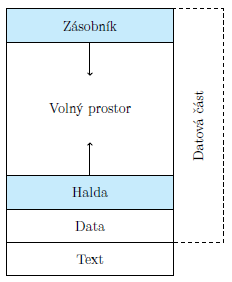
\includegraphics[width=\textwidth]{images/proc_user_context.png}
    \caption{Uživatelský kontext procesu}
  \end{minipage}
  \hfill
  \begin{minipage}[b]{0.4\textwidth}
    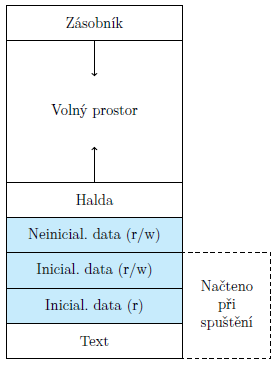
\includegraphics[width=\textwidth]{images/proc_data_segment.png}
    \caption{Datová část paměti procesu}
  \end{minipage}
\end{figure}

Datový segment lze rozdělit:

\begin{itemize}
    \item  Inicializovaná data dostupná pouze pro čtení – datové prvky inicializované programem,
    které nelze měnit.
    \item Inicializovaná data dostupná pro čtení i zápis – datové prvky inicializované programem,
    ovšem jejich hodnoty mohou být za běhu procesu měněny.
    \item Neinicializovaná data – datové prvky, které program neinicializoval. Neinicializovaná
    data lze měnit za běhu procesu.
\end{itemize}

\begin{Large}
    \vspace{0,5cm}
    \textbf{Kontext jádra}
\end{Large}

Informace potřebné pro správu procesů se mohou nacházet v \textit{řídící tabulce procesů - PCB (Process Control Block)}. V této tabulce jsou obsaženy informace o všech procesech, které jsou spuštěny. PID identifikátor navíc funguje v tabulce jako index procesu. 

\vspace{0,5cm}

V tomto kontextu jsou udržovány informaci o rozložení uživatelského kontextu, dále udržuje informace o jeho správě:
\begin{itemize}
    \item Programový čítač - obsahuje adresu následující instrukce procesu, která bude vykonána procesorem
    \item Parametry spojené s plánováním běhu procesů - priorita procesu, čas aktivity v CPU, ukazatel na plánovací frontu atd. Tyto informace jsou použity při plánování procesů, tj. rozhodování, který proces je na řadě. 
    \item Seznam vstupů a výstupů využívané procesem - například se může jednat o seznam otevřených souborů
    
    \newpage
    
    \item Stav činnosti procesu (zjednodušeně):
    \begin{enumerate}
        \item Nový - proces je vytvářený
        \item Připravený - proces čeká na to, až mu bude přidělen procesor
        \item Vykonávaný/prováděný - instrukce jsou prováděny\footnote{V tomto stavu může být vždy jenom jeden proces! Ale více programů může být ve stavu \textit{připravený} nebo \textit{čekající}}
        \item Čekající - proces čeká na nějakou událost, jako načtení dat
        \item Ukončený - proces dokončil vykonávání instrukcí
    \end{enumerate}
\end{itemize}

Po vytvoření procesu je ve stavu \textit{připravený}. Poté co je vybrán plánovačem procesů tak je \textit{vykonáván}. Vykonávání se ukončí buď dobrovolným opuštěním procesu, nebo v případu příchozího přerušení, nebo zablokování procesu z důvodu čekání na určitou událost (například na načítající se data). Při zablokování, poté co proces již není ve stavu \textit{čekání} je opět ve stavu \textit{připravený}. A celý $"$cyklus$"$ se opakuje. Pokud proces svou práci dokončí, tak přejde do stavu \textit{ukončený} do kterého lze přejít pouze ze stavu \textit{vykonávaný}! Při změně vykonávání procesu - přepnutí kontextu - se aktuální stav běhu procesu uloží v řídící tabulce procesů, ze které se i načítá poslední stav běhu procesu.

\begin{center}
    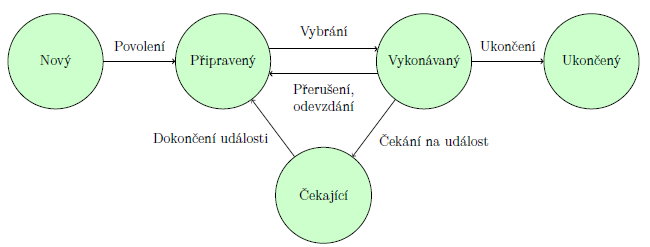
\includegraphics[scale=1]{images/proc_states.png}
\end{center}

\begin{Large}
    \vspace{0,5cm}
    \textbf{Vlákna}
\end{Large}

Lze si je představit jako stavební bloky procesů, které jsou jím vykonávané. Proces může mít jedno i více vláken, kde každé vlákno umožňuje procesu provádět pouze jeden úkol v daném čase. Je pak tedy zřejmé, že více vláken může vykonávat více různých úkolů nebo dokonce jeden stejný úkol nad různými daty (například u webového serveru). Zároveň, aby tyto úkoly šlo vykonávat ve stejném čase, musí být přítomno buď více procesorů, nebo více jader v procesoru (jedno jádro resp. jeden procesor vykonává jedno vlákno). Důležité je si zapamatovat, že každé vlákno má vlastní zásobník, ale sdílí zbytek uživatelského kontextu! (tj. datový i textový segment a haldu)

\vspace{0,5cm}

Právě skrz sdílený uživatelský kontext vláken je třeba aby programátor zajistil hladký průběh paralelizace. Například při sdílení dat mezi vlákny může dojít ke čtení nekonzistentních dat tj. k souběhu (viz \ref{sync}). 

\vspace{0,5cm}

Poté z pohledu spravování vláken je lze rozdělit na dva typy, \textit{vlákna jádra} (z programu jádra) a \textit{uživatelská vlákna} (z programů mimo jádro). Mezi uživatelskými vlákny a vlákny jádra existuje několik možných návazností/modelů:

\begin{center}
    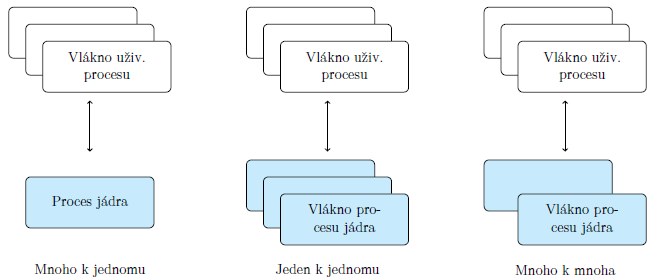
\includegraphics[scale=1]{images/thread_models.png}
\end{center}

\begin{itemize}
    \item Mnoho k jednomu - K více uživatelských vláknům přiřazuje jeden proces jádra. Použití vláken není závislé na jejich podpoře v OS a jejich správa je zajištěna často v podobě \textit{vláknových knihoven} (v uživatelském režimu). Tyto knihovny vytváří, plánují běh, přepínají a ruší vlákna. Nevýhodou je, že zavolání blokujícího sys. volání jedním z vláken zablokuje celý proces (tedy všechny vlákna), jelikož jádro nepracuje s vlákny.  
    \item Jeden k jednomu - Každé uživatelské jádro má korespondující vlákno v jádře a tedy má i na starosti jejich správu. Výhodou je, že blokující sys. volání neblokuje všechny ostatní vlákna. Dále je umožněn běh paralelně na více procesorech. Nevýhodou je značná režie, skrz vysoké množství vláken.
    \item Mnoho k mnoha - Kombinace předešlých, přiřazuje vláknům stejný nebo menší počet vláken v kernelu. Počet těchto vláken může být omezen vzhledem k aplikaci nebo druhu zařízení (např. jednoprocesorové vs. víceprocesorové)
\end{itemize}

%%%%%%%%%%%%%%%%%%%
% ČINNOST PROCESŮ %
%%%%%%%%%%%%%%%%%%%

\newpage
\section{Činnost procesů\,--\,stavy činnosti, rozšířený stavový model běhu procesů} \label{proces-work}

Dříve vyjmenované stavy nejsou kompletní výčet. Skutečný stavový model má devět položek, které jsou:

\begin{enumerate}
    \item Proces je vykonáván v uživatelském režimu
    \item Proces je vykonáván v režimu jádra
    \item Proces je připraven ke zpracování a je uložen v hlavní paměti
    \item Proces je spící a je uložen v hlavní paměti
    \item Proces je připraven ke zpracování a je uložen v odkládací paměti
    \item Proces je spící a je uložen v odkládací paměti
    \item Vykonávání procesu je nuceně přerušeno
    \item Proces je vytvořený a je v přechodovém stavu
    \item Proces je ve stavu \textit{zombie}, neexistuje, ale v systému je o něm záznam 
\end{enumerate}

\begin{center}
    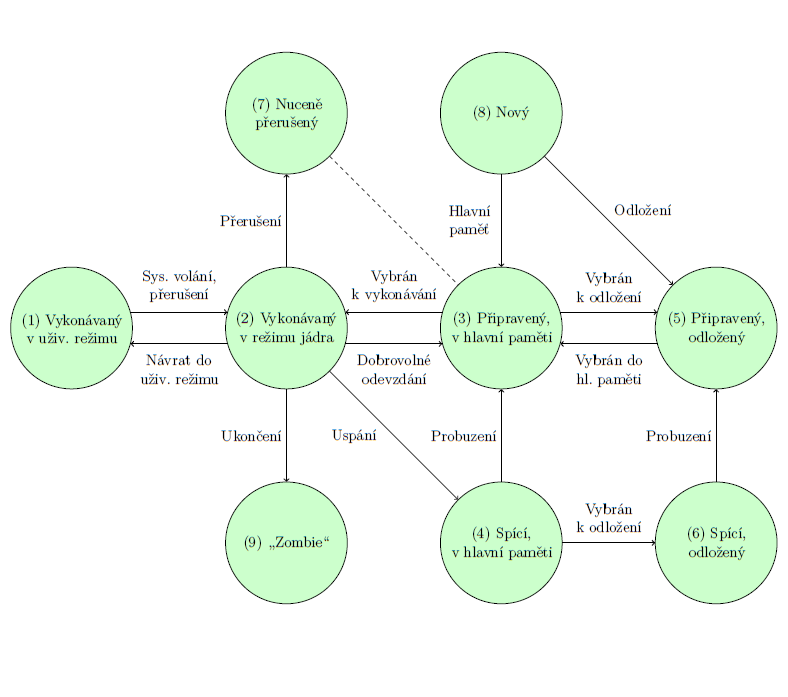
\includegraphics[scale=0.9]{images/proc_extended_states.png}
\end{center}

Je důležité si povšimnout, že se prakticky jedná o rozšíření zkráceného modelu. Například stav \textit{vykonávaný} je zde rozšířen o informaci v jakém režimu běží. A jaký je rozdíl mezi \textit{uživatelským režimem} a \textit{režimem jádra}? Do režimu jádra se proces dostane pomocí systémových volání nebo přerušení, jinak (s výjimkou jádru vlastních procesů) běží v uživatelském režimu!

\vspace{0,5cm}

Stav \textit{čekající} je zde rozšířen na \textit{spící a uložen v hlavní paměti} a \textit{spící a uložen v odkládací paměti}. Přechod mezi těmito dvěma stavy řídí plánovač II. úrovně, který vyměňuje procesy mezi hlavní (RAM) a odkládací pamětí (swap na disku). Změna stavu zde může být pouze do odkládací paměti. 

\vspace{0,5cm}

\textit{Připravený} je nahrazen stavy \textit{připravený ke zpracování a uložen v hlavní paměti} a \textit{připraven ke zpracování a uložen v odkládací paměti}. Přechod je zde opět dán plánovačem II. úrovně. Tentokrát však dochází k obousměrným přechodům. 

\vspace{0,5cm}

\textit{Proces v hlavní paměti} zahrnuje stavy \textit{připraven ke zpracování a uložen v hlavní paměti} a \textit{spící a uložen v hlavní paměti}. Přechod mezi těmito stavy je jednosměrný a je způsoben probuzením procesu (dočkáním se na událost kvůli které byl uspán).

\vspace{0,5cm}

\textit{Proces v odkládací paměti} zahrnuje stavy \textit{připraven ke zpracování a uložen v odkládací paměti} a \textit{spící uložen v odkládací paměti}. Přechod funguje stejně jako v předešlém odstavci. 

\begin{Large}
    \vspace{0,5cm}    
    \textbf{Více do hloubky}
\end{Large}

\begin{large}
    \vspace{0,5cm}
    \textbf{Vytvoření procesu}
\end{large}

Proces vzniká pomocí sys. volání \textit{fork} kde z původního procesu (\textit{rodič}) se vytvoří nový proces (\textit{potomek}). Pro možnost identifikace rodiče potomka se zavádí identifikátor \textit{PPID} (Parent Process IDentifier), zároveň zpravidla platí, že proces má jednoho rodiče, ale rodič může mít více potomků\footnote{Všechny procesy jsou následovníkem procesu \textit{init}.}. 

\vspace{0,5cm}

Sys. volání \textit{fork} je voláno rodičem jednou a vráceno dvakrát. Vrací se PID rodiče a PID 0 pro potomka (zjednodušuje rozlišení potomka a rodiče při programování), potomek následně volá sys. volání \textit{execve}, kterým spustí programový kód nového procesu. Ale co paměť, procesu? \textit{Fork} vytvoří kopii rodičovského procesu, existují pak tedy dva stejné procesy.

\vspace{0,5cm}

\textit{Fork} je vykonáván v režimu jádra, zde se vyhledá volná pozice v tabulce procesů a obsadí se záznamem potomka (jeho kontext jádra, viz \ref{procesy}) a poté se alokuje paměť pro uživatelský kontext potomka (taktéž v kapitole \ref{procesy}) který se naplní kopií uživatelského kontextu rodiče\footnote{Textová část může být buď kopírována nebo sdílena.}. Proces skončí jakmile dokončí svůj kód a vyvolá sys. volání pro své ukončení (např. \textit{exit}). Proces však nemusí ukončit jen sám sebe, pokud má dostatečná oprávnění může ukončit i jiný proces. Po ukončení procesu je rodiči navrácen PID ukončeného procesu. 

\vspace{0,5cm}

Proces může ze stavu $"$vytvořený$"$ přejít do stavu $"$připraven na zpracování$"$, záleží však kolik je volného místa v paměti. Pokud je ho dost, tak přejde do stavu $"$připraven ke zpracování v hlavní paměti$"$ kde čeká až jej vybere plánovač I. úrovně a pak přejde do stavu $"$vykonávaný v režimu jádra$"$ kde se obslouží sys. volání. Nakonec přejde do režimu $"$vykonáván v uživatelském režimu$"$.

\begin{large}
    \vspace{0,5cm}
    \textbf{Vykonávání procesu}
\end{large}

Už víme, že proces je vykonáván buď v režimu jádra nebo v uživatelském režimu, kde přechází do režimu jádra pomocí volání sys. volání a obsluhy přerušení. Je však třeba podotknout, že procesy se nestřídají pouze po dokončení práce, nebo při dobrovolném čekání. Může totiž docházet i k preemptivnímu střídání procesů, kdy každý proces má povolenou maximální dobu vykonávání. Pokud tato doba uběhne, je proces přerušen a přejde do stavu $"$nuceně přerušený$"$ (který je totožný se stavem \textit{připraven na zpracování v hlavní paměti}\footnote{Jediný rozdíl je v tom jak se proces do tohoto stavu dostal.}). Plánovač pak vybere jiný proces k vykonávání. 

\vspace{0,5cm}

Druhou možností je, že proces se dobrovolně ukončí před uplynutím maximálního časového intervalu a opět přejde do stavu \textit{připraven ke zpracování v hlavní paměti}.

\begin{large}
    \vspace{0,5cm}
    \textbf{Uspání procesu}
\end{large}

Předpokládejme, že aby proces mohl pokračovat ve svém úkolu, tak musí počkat na vstupně/výstupní (I/O - Input/Output) operaci. Proces zavolá systémové volání pro zápis/čtení dat a přejde ze stavu \textit{vykonáván v uživatelském režimu} do stavu \textit{vykonáván v režimu jádra}. Aby proces neplýtval zdroje čekáním v tomto stavu, tak se sám zablokuje (\textit{uspí}) a přejde do stavu \textit{spící v hlavní paměti}. Tímto uvolní místo pro jiný proces čekající v hlavní paměti. 

\vspace{0,5cm}

Po dokončení, v tomto případě, vstupně/výstupní operace je proces probuzen a je připraven v hlavní paměti. Zde čeká až jej vybere Plánovač I. úrovně. 

\begin{large}
    \vspace{0,5cm}
    \textbf{Odložení procesu}
\end{large}

Pokud je v systému spuštěno tolik procesů, že se nevejdou do hlavní paměti přichází na řadu Plánovač II. úrovně (tzv. vyměňovací proces), který vybere proces k přesunutí z hlavní paměti do odkládací paměti (\textit{připravený v hlavní paměti} $\xrightarrow{}$ \textit{připravený, odložený}). Stejně tak může přesouvat spící procesy z hlavní paměti do odkládací paměti. Po probuzení jej může Plánovač opět přesunout zpět do hlavní paměti.

\vspace{0,5cm}

Je třeba mít na vědomí, že plánovač II. úrovně vybírá procesy tak aby se všechny vystřídaly v hlavní paměti. Tam pak čekají na plánovač I. úrovně. 

\begin{large}
    \vspace{0,5cm}
    \textbf{Ukončení procesu}
\end{large}

Proces ve uživatelském režimu zavolá sys. volání (např. dříve zmíněný \textit{exit}), přejde tedy do režimu jádra a dále do stavu \textit{zombie}. V tomto stavu proces neexistuje, ale je o něm stále udržován záznam v tabulce procesů. Jakmile rodič zpracuje informaci o jeho ukončení, tak je proces definitivně ukončen. 

%%%%%%%%%%%%%%
% SCHEDULING %
%%%%%%%%%%%%%%

\newpage
\section{Plánování procesů\,--\,okamžiky rozhodnutí, plánovací algoritmy, systém priorit} \label{planning}

V dnešní době se plánování procesů (\textit{scheduling}) musí plánovat na více procesorech a jádrech. Jak tedy zajistit, že každý proces dostane procesorový čas a nebude žádný vynechán? Proto přichází na řadu plánovač (\textit{process scheduler}) a plánovací algoritmy. Tyto se využívají za účelem navození pocitu, že vše v Operačním Systému běží současně, přitom se jedná o neustálé a rychlé přepínání kontextu.

\begin{Large}
    \vspace{0,5cm}
    \textbf{Okamžiky rozhodnutí}
\end{Large}

Okamžiky kdy se plánovač musí rozhodnout, který proces bude vykonáván jsou následující:
\begin{enumerate}
    \item Vytvoření procesu - bude se vykonávat rodič nebo potomek?
    \item Ukončení procesu - který proces jej nahradí?
    \item Blokování procesu - při čekání na I/O operaci, který proces jej nahradí?
    \item Přerušení procesu - a) přerušení od zařízení b) přerušení od hodin; který jej nahradí?
\end{enumerate}

Průběh při výkonu dvou procesů, lze jednoduše ukázat na následujícím obrázku. Procesy se střídají podle toho, který zrovna čeká (např. na I/O operaci). Při přerušení může dojít k rozhodnutí o přepnutí procesu, přerušení od hodin může také být signál pro rozhodnutí o přepnutí procesu. Toto přepnutí může být provedeno při každém \textit{n-tém} přerušení. 
\vspace{0,5cm}
Dále je třeba rozlišit jestli je systém nepreemptivní (kooperativní) či preemptivní. V prvním případě dochází ke přepínání pouze pokud proces dobrovolně uvolní procesor. Ve druhém případě (preemptivní) se přepíná na základě nuceného přerušení od hodin, kdy pak plánovač zvolí jiný proces k vykonávání. 

\begin{center}
    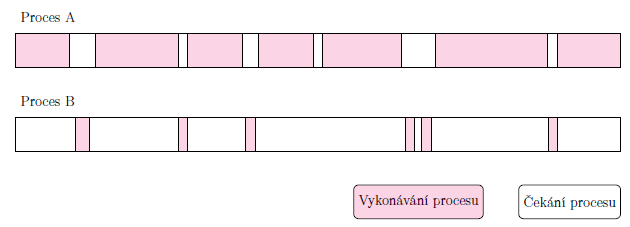
\includegraphics[scale=1]{images/proc_changing.png}
    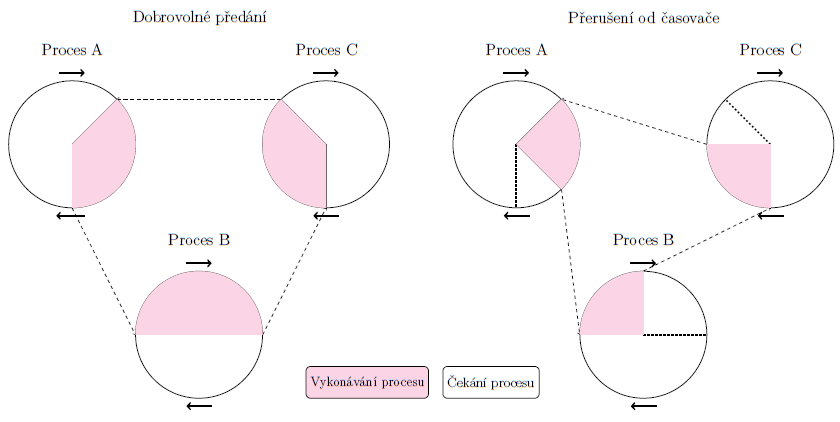
\includegraphics[scale=1]{images/proc_preemption.png}
\end{center}

\begin{Large}
    \textbf{Typy plánovacích algoritmů}
\end{Large}

I když nám to tak mže připadat, tak ne všechny počítače mají stejný účel, například letové systémy vyžadují co nejrychlejší odezvu v určeném časovém úseku na rozdíl od našeho domácího počítače, který upředostňuje komfort a ne splňování \textit{deadlinů}.

\begin{large}
    \vspace{0,5cm}
    Dávkové systémy
\end{large}

Tj. \textit{Batch} systémy, zpracovávají úkoly v tzv. dávkách bez účasti uživatele. Tímto jsou eliminovány prodlevy způsobené čekáním na akce od uživatele. Používá se nepreemptivních plánovačů (tedy proces sám musí uvolnit procesor). 

\vspace{0,5cm}

Tyto systémy jsou typické pro nákladné a výkonné informační centra, kde je prioritou co nejlépe využít drahý hardware. Sledují se především tyto parametry:

\begin{itemize}
    \item Výkonnost - počet úloh zpracovaných za jednotku času\footnote{Pozor, plánovač co zvyšuje výkonnost nemusí nutně zvyšovat rychlost obsluhy. Za účelem zvýšení výkonnosti může upřednostňovat kratší úlohy, na které se však musí déle čekat. Výkonnost stoupá, ale rychlost obsluhy klesá.} 
    \item Rychlost obsluhy - průměrný čas od doby přijetí požadavku do jeho splnění
    \item Využití CPU - preferuje se maximální využití a minimální prostoje
\end{itemize}

Například systémy od IBM a GCOS (General Comprehensive Operating System) od firmy Bull SAS.

\begin{large}
    \vspace{0,5cm}
    Interaktivní systémy
\end{large}

Zde je chod systému ovlivňován uživatelem a právě jeho požadavky by měly být vyřizovány přednostně. Uživatel předpokládá, že program který má právě v popředí bude pracovat co nejrychleji a stejně tak reagovat, interaktivní systémy se snaží tento předpoklad splnit. Plánovač sice nemůže ovlivnit složitost úlohy a rychlost zpracování, může však přispět ke splnění očekávání uživatele. Je zřejmé, že se upřednostňuje užívání preemptivního přepínání, aby nemohl žádný proces zabrat CPU na příliš dlouhou dobu. 

\vspace{0,5cm}
Co se sleduje?
\begin{itemize}
    \item Čas odezvy - čas od vyslání příkazy po obdržení výsledku
    \item Přiměřenost - přiměřenost složitosti úlohy k době jejího zpracování
\end{itemize}

\vspace{0,5cm}

Jedná se o klasické desktop systémy, jako Windows, MacOS a různé distribuce OS Linux. 

\begin{large}
    \vspace{0,5cm}
    Real-Time systémy
\end{large}

Používají se pro zpracování úloh, které slouží jako vstup dalších navazujících činností. Tyto systémy musí splnit úlohu v reálném čase (v předem daném časovém úseku). Tyto systémy jsou používány v automatizovaných procesech, robotice a také telekomunikacích. Používá se opět preemptivní plánování. 

\vspace{0,5cm}

Podle toho jak moc se tlačí na splnění požadavků v daném času můžeme tyto systémy dělit:

\begin{itemize}
    \item \textit{hard} - časové záruky jsou pouze přibližné, určité časové odchylky jsou povoleny.
    \item \textit{soft} - časové záruky jsou plně zajištěny. 
\end{itemize}

\vspace{0,5cm}

Sledujeme parametry:

\begin{itemize}
    \item Dodržování časových termínů - nejdůležitější požadavek!!
    \item Předvídatelnost/pravidelnost - například u systémů pro zpracování multimediálních dat.
\end{itemize}

\vspace{0,5cm}
Příkladem real-time systémů jsou FreeRTOS (open source\footnote{\url{https://github.com/FreeRTOS/FreeRTOS}}) a VxWorks od firmy Wind River. 

\vspace{0,5cm}

Na základě znalosti času který je potřeba pro obsloužení periodických událostí můžeme prohlásit, zda je systém schopný činnosti. Mějme \textit{m} periodických událostí, kde se událost \textit{i} vyskytuje s periodou $\mathrm{P_i}$ a vyžaduje $\mathrm{C_i}$ procesorového času. Aby real-systém byl běhu schopný, musí splňovat následující podmínku:

\begin{equation}
    \sum\limits_{i=1}^m \frac{C_i}{P_i} \leq 1 \nonumber \nonumber 
\end{equation}

\newpage

\begin{Large}
    \vspace{0,5cm}
    \textbf{Systém priorit}
\end{Large}

Plánovač I. úrovně vybírá procesy, které jsou připravené a v hlavní paměti aby získali procesorový čas. Algoritmus plánování je postaven na \textit{paralelních frontách}, kde každá fronta je spojena s intervalem priorit. Uživatelské procesy mají kladnou prioritu (na UNIX,Linux) a procesy jádra mají záporné hodnoty (opět UNIX, Linux). Z toho vyplývá, že nižší hodnota znamená vyšší prioritu (takže procesy jádra mají nejvyšší prioritu - obsluhují sys. volání).  

\vspace{0,5cm}

Plánovač prochází fronty od nejnižších intervalů (nejvyšší priorita) dokud nenalezne obsazenou frontu. Poté vybere první proces z dané fronty a po vykonání je proces vložen na konec místní fronty (round-robin). Priorita každého procesu je počítána (pro začátek každého intervalu, např. každou sekundu) pomocí následujícího vzorce:

\begin{equation}
    P = V + N + B \nonumber \notag
\end{equation}

Podle této nové priority je proces přiřazen do fronty. Fronta bývá zvolena na základě dělení vypočtené priority zvolenou konstantou. 

\vspace{0,5cm}

\textit{V} je prakticky prostě čítač, představující využití procesoru. Tato hodnota se inkrementuje s každým taktem procesorových hodin (pokud je proces vykonáván na procesoru). Tímto způsobem se upřednostňují nové procesy, které ještě nezískali procesorový čas. Zároveň lze procesy co zrovna využily procesor penalizovat pomocí navýšení původní hodnoty \textit{V} o aktuální hodnotu z daného intervalu a výsledek je vydělen dvěma. Tímto způsobem jsou penalizovány nedávno vykonané procesy a předchází se \textit{stárnutí procesů}.

\vspace{0,5cm}

Hodnota \textit{N} (tj. \textit{nice}) je implicitně nastavena na 0 (povolený rozsah je -20 až +19). Tato hodnota je zděděna od rodičovského procesu.

\begin{itemize}
    \item Běžný uživatel může nastavovat hodnoty 0 - 19, čímž může vlastní procesy penalizovat.
    \item Administrátor může procesy \textit{preferovat} snížením hodnoty \textit{N} v rozmezí -20 až -1.
\end{itemize}

\vspace{0,5cm}

\textit{B} tj. \textit{báze} je použita pokud se proces zablokuje (např. protože čeká na I/O operaci), proces je tedy odstraněn z plánovací fronty (jelikož není ve stavu \textit{připraven}). Až se dočká události, je znovu zařazen do fronty, ale s jinou prioritou. Volba fronty/priority závisí na události, na kterou proces čekal (nastaví se hodnota B).

%%%%%%%%%%%%%%%%%
% SYNCHRONIZACE %
%%%%%%%%%%%%%%%%%
\newpage
\section{Synchronizace procesů\,--\,souběh, vzájemné vyloučení, uvíznutí procesů} \label{sync}

Zajištění synchronizace je zásadní problém v jakémkoliv paralelně běžícím systému. Jeden proces může svým během ovlivnit jiný proces nebo jím být ovlivněn, aby k tomu nedošlo zavádíme synchronizační techniky. Čeho tím chceme docílit? 
\begin{enumerate}
    \item Vyloučení konfliktu kritických činností pro zamezení souběhu
    \item Zajištění časové souslednosti pro paralelní programování
\end{enumerate}

\begin{Large}
    \vspace{0,5cm}
    \textbf{Souběh}
\end{Large}

Nastává při práci procesů se sdílenými prostředky. Například si představme frontu pro tiskárnu s ukazatelem \textit{in} ukazující poslední volné místo ve frontě a dva procesy A a B. Proces A načte z fronty že první volné místo je na pozici 10 a tuto informaci uloží do lokální proměnné. Následně však plánovač přepne kontext na proces B, který udělá to stejné a uloží svůj soubor na index 10 a inkrementuje jej na 11. Plánovač poté přepne kontext zpět na proces A, který má stále uloženou hodnotu 10! Tedy přepíše soubor procesu B! 

\begin{center}
    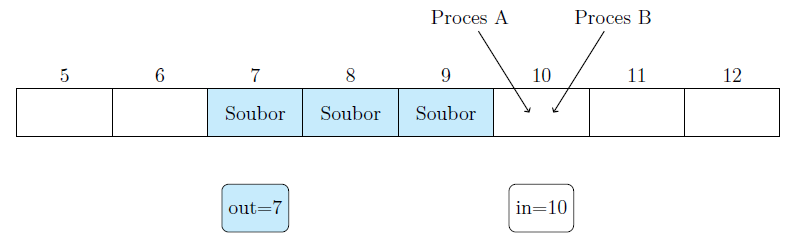
\includegraphics[scale=1]{images/proc_soubeh.png}
\end{center}

Toto čtení nekonzistentních dat z důvodu přepnutí kontextu nazýváme \textit{souběh} tj. \textit{race condition}. Problémem je, že k souběhu nemusí vždy dojít, záleží čistě na plánovači a kdy dojde k přepnutí kontextu, proto se tato chyba velmi špatně zachytává při testování. 

\begin{large}
    \vspace{0,5cm}
    \textbf{Zajištění časové souslednosti}
\end{large}

Používá se, když proces musí čekat na dokončení celé množiny operací, než může pokračovat. Toho lze docílit pomocí paralelního programování za využití vláken a tzv. \textit{bariér}/\textit{časové mezníky}. 

\vspace{0,5cm}

Představme si aplikaci používající vlákna. Všechny vlákna musí dokončit svou úlohu z fáze 1 než mohou přejít do fáze 2 a i když vlákna vykonávají stejný kód, tak mohou pracovat různými rychlostmi. Pokud nějaké vlákno skončí s úlohou z fáze 1 dřív jak jiné, bude pozastaveno než je dokončí všechny ostatní vlákna.

\begin{center}
    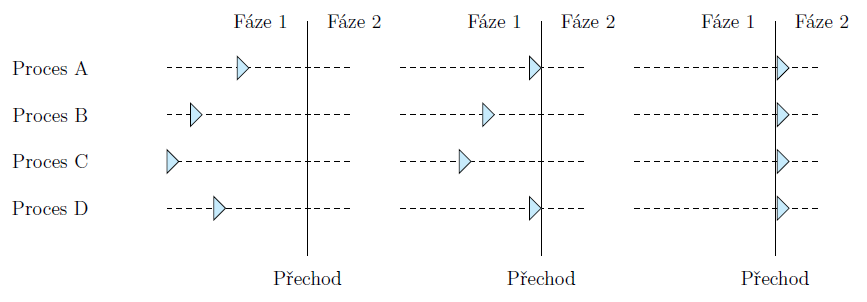
\includegraphics[scale=1]{images/proc_barrier.png}
\end{center}

\begin{large}
    \vspace{0,5cm}
    \textbf{Vzájemné vyloučení pomocí kritické sekce}
\end{large}

Souběhu lze zabránit výlučným přístupem ke sdílenému prostředku, tedy že dokud jeden proces pracuje se sdíleným prostředkem ostatní jsou zablokované a čekají na uvolnění prostředku. Tohoto lze docílit například pomocí určení části kódu, kterou označíme za \textit{kritickou sekci} ve které se smí nacházet vždy nanejvýše jeden proces. 

\vspace{0,5cm}

Této myšlence se obecně říká \textit{zámek} (tj. \textit{mutex}), tedy že přístup ke sdílené proměnné je uzamčen pro ostatní procesy. Mezi často používané patří například semafory. Proces zkontroluje zámek, pokud je \textit{odemčený} \textit{uzamče} jej a přistoupí k proměnné (vstoupí do kritické sekce). Po dokončení operací zámek \textit{odemče} a umožní přístup ostatním procesům. 

\vspace{0,5cm}

Krom vzájemné vyloučení je potřeba zajistit i následující podmínky:
\begin{enumerate}
    \item Blokování jiného procesu je pouze možné v případě, že jiný proces je v kritické sekci. Blokování procesem mimo KS je nepřijatelné. 
    \item Doba čekání na vstup do kritické sekce musí být konečná
\end{enumerate}

\begin{large}
    \vspace{0,5cm}
    \textbf{Vzájemné vyloučení pomocí proměnných}
\end{large}

\begin{itemize}
    \item sdílená dvouhodnotová proměnná
    \item striktní střídání procesů
\end{itemize}

\begin{large}
    \vspace{0,5cm}
    \textbf{Sdílená dvouhodnotová proměnná}
\end{large}

Mějme sdílenou proměnnou \textit{lock}, která může nabývat stavů \textit{FALSE} a \textit{TRUE}. \textit{FALSE} značí, že v kritické sekci není žádný proces a \textit{TRUE} značí obsazenou kritickou sekci. Procs tedy před vstupem do KS zkontroluje proměnnou a postupuje tak jak bylo popsáno dříve. Pokud je \textit{lock} uzamčený (\textit{TRUE}) proces čeká v čekající smyčce\footnote{Tomuto se říká aktivní čekání a jedná se o skvělý způsob jak plýtvat zdroji.} na uvolnění prostředků. 

\vspace{0,5cm}

Problémem je však skutečnost, že tento způsob je náchylný na souběh. Může se stát, že proces A přistoupí k \textit{lock} a načte jeho hodnotu jako \textit{FALSE}, poté plánovač přepne kontext na proces B který vstoupí do kritické sekce, a nastaví \textit{lock} na \textit{TRUE}.  Plánovač opět přepne kontext a proces A vstoupí do kritické sekce, výsledkem jsou dva procesy v kritické sekci najednou. 

\begin{large}
    \vspace{0,5cm}
    \textbf{Striktní střídání procesů}
\end{large}

Opět může být docíleno pomocí sdílené dvou-stavové proměnné, např. \textit{turn} nabývající hodnot 0 a 1 (0 = A, 1 = B). Pokud je zrovna hodnota 0, tak proces A může vstoupit do KS a proces B je v čekací smyčce. Po dokončení práce procesu A, je \textit{turn} nastaven na 1.

\vspace{0,5cm}

Problém nastává když jeden z procesů vstupuje do KS častěji jak druhý. Pak je například hodnota \textit{turn} nastavena na 1 a proces A musí čekat na proces B, který však zatím ani v KS není. Tímto se porušilo pravidlo, že proces může být blokován pouze procesem v kritické sekci. 

\begin{large}
    \vspace{0,5cm}
    \textbf{Vzájemné vyloučení pomocí hardwarových funkcí}    
\end{large}

\begin{itemize}
    \item zákazem přerušení
    \item atomickými instrukcemi
\end{itemize}

\begin{large}
    \vspace{0,5cm}
    \textbf{Zákazem přerušení}    
\end{large}

Toto řešení platí pro preemptivní systémy, kde se zákazem přerušení na procesoru zajistí, že proces nelze přerušit dokud nevystoupí z kritické sekce. Přerušení mohou obecně zakazovat uživatelské i systémové programy, ovšem povolit zakazování přerušení pro uživatelský program je velmi riskantní. 

\vspace{0,5cm}

Tento přístup však funguje pouze na jednoprocesorových systémech. Pokud je procesorů více, tak na jednom je přerušení sice zakázáno, ale tento zákaz neplatí pro procesy na ostatních procesorech. Zavedení zákazu přerušení na všech procesorech by vyžadovalo zaslání zprávy všem procesorům, což je časově neefektivní operace. 

\begin{large}
    \vspace{0,5cm}
    \textbf{Atomickými instrukcemi}    
\end{large}

Jedná se o instrukce, které umožní číst a měnit hodnotu (nebo zaměnit obsah dvou proměnných) a nelze je přerušit. Princip lze pochopit na instrukci \textit{TestAndSet} (tj. \textit{TSL - Test and Set Lock}). Tato instrukce testuje proměnnou, pokud je nastavena na FALSE nastaví na TRUE a proces vstoupí do KS. Ostatní procesy potom čekají v aktivní smyčce (opakovaně volají \textit{TestAndSet} dokud není \textit{lock} opět FALSE). Poté co proces skončí v KS nastaví proměnnou na FALSE. 

\vspace{0,5cm}

Princip je podobný jako u přístupu se sdílenou proměnnou, krom toho že instrukce je nepřerušitelná, tedy nemůže dojít k přepnutí kontextu a tím pádem k souběhu. 

\begin{large}
    \vspace{0,5cm}
    \textbf{Vzájemné vyloučení pomocí sys. volání}    
\end{large}

Předešlé metody využívají aktivního čekání, které má následující nevýhody:
\begin{itemize}
    \item Plýtvání časem CPU\footnote{Pokud je předpoklad, že se nebude čekat moc dlouho, jde využít aktivního čekání.}
    \item Porušení základní podmínky, že čekání na vstup do kritické sekce musí být konečná.
\end{itemize}

Další problém se kterým se můžeme u paralelizmu setkat, je \textit{problém opačné priority}. Pokud máme dva procesy, kde proces A má vyšší prioritu jak B a proces B je v kritické sekci. Plánovač zvolí k vykonání proces A (s vyšší prioritou), který čeká na přístup do KS. Jelikož je však procesu A dávána přednost, tak proces B nikdy z KS nevystoupí. 

\vspace{0,5cm}

Jak lze tento problém vyřešit? Procesy se mohou navzájem uspávat, v tomto případě by tedy proces A uspal B a zaslal by mu signál na probuzení až po výstupu z KS. I zde však může nastat souběh. Toto lze ilustrovat na tzv. \textit{producer-consumer problem}, kde máme dva procesy, jednoho producenta a spotřebitele. Procesy pracují se sdílenou pamětí o omezené velikosti, producent paměť naplňuje a jakmile je plná tak přejde do režimu spánku, následně spotřebitel odebere položku z paměti, čímž probudí producenta. Pokud chce spotřebitel odebrat z paměti a je prázdná tak se uspí. Ke sledování stavu v paměti se může použít sdílené proměnné (\textit{counter}) a komunikace probíhá pomocí sys. volání.

\vspace{0,5cm}

Pokud je paměť prázdná (tedy \textit{counter = 0}) spotřebitel přečte hodnotu sdílené proměnné, ale před uspáním dojde k přepnutí kontextu. Producent uvidí, že paměť je prázdná a začne ji naplňovat. Jakmile zvýší proměnnou o jedna zavolá sys. volání aby probudil spotřebitele (v domnění že je uspaný), tím že spotřebitel nespí nemá volání žádný účinek. Producent tedy kompletně naplní paměť a uspí se. Dojde k přepnutí kontextu a spotřebitel se také uspí. Došlo tedy k \textit{fatálnímu souběhu}. 

\begin{large}
    \vspace{0,5cm}
    \textbf{Uvíznutí tj. deadlock}    
\end{large}

Skupina procesů je ve stavu uvíznutí, pokud každý z nich čeká na událost, kterou může způsobit pouze jiný proces z této skupiny. Uvíznutí může nastat nad různými prostředky (hardwarové či softwarové), které dělíme na \textbf{sdílitelné} (globální proměnné, sdílený úsek paměti, záznam v databázi, ...) a \textbf{nesdílitelné} (tiskárny, scannery, DVD, ...). Sdílené prostředky mohou být uzamčené. Dále lze rozdělit na \textbf{přepínatelné}\footnote{Uvíznutí nenastává nad sdílitelnými prostředky bez jejich uzamčení, nebo nad přepínatelnými prostředky kde lze uvíznutí předejít předáním jinému procesu.} a \textbf{nepřepínatelné}\footnote{Odebrání přepínatelného prostředku nezpůsobí žádnou škodu - např. hlavní paměť. Nepřepínatelný prostředek je takový, jehož odebrání způsobí nefunkčnost procesu.}. 

\vspace{0,5cm}

Využití sdíleného prostředku se skládá ze tří částí:
\begin{enumerate}
    \item Žádost - Proces žádá o využití prostředku a aktivně čeká pokud je využitý
    \item Používání - Proces využívá prostředek
    \item Uvolnění - Proces ukončil práci a předal o tom zprávu
\end{enumerate}

Důvody k uvíznutí mohou být například, že první proces čeká na prostředek obsazený druhým procesem, který je také ve stavu čekání na prostředek obsazený prvním procesem (obrázek níže). Často se jedná i o chybu v programu při předávání informace o využívání prostředku.

\begin{center}
    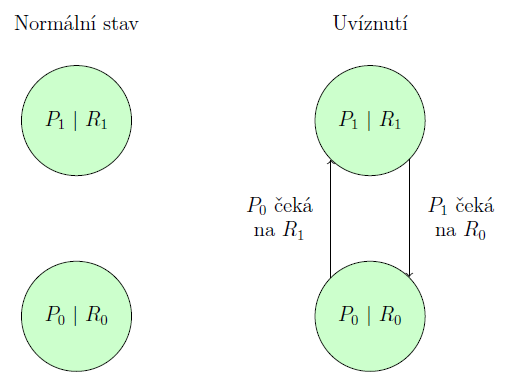
\includegraphics[scale=1]{images/proc_deadlock.png}
\end{center}

Tato situace se řeší (v různých OS) následovně:
\begin{itemize}
    \item Předcházení uvíznutí
    \item Připuštění, že se systém dostane do stavu uvíznutí, ale se schopností tento stav detekovat a obnovit nomální činnost
    \item Ignorovat tento problém
\end{itemize}

Detekce a napravení deadlocku vyžaduje neustálé spouštění algoritmu se dvěma metodami obnovení činnosti:

\begin{itemize}
    \item Procesy ve stavu uvíznutí jsou násilně ukončeny: 
    \begin{enumerate}
        \item postupně - pomalejší řešení, po každém ukončeném procesu je potřeba znovu spustit detekční algoritmus, volba procesu může být například na základě stáří
        \item všechny najednou - rychlejší řešení s velkými náklady (například ztráta předešlých výpočtů a dat)
    \end{enumerate}
    
    \item Procesům jsou násilně odebrány všechny prostředky a předávány jiným procesům ve stavu uvíznutí- Po každém odebrání je opět potřeba spustit detekční algoritmus, aby se zjistilo zda bylo uvíznutí vyřešeno.
\end{itemize}

%%%%%%%%%%%%%%%%%
% SPRÁVA PAMĚTI %
%%%%%%%%%%%%%%%%%

\newpage
\section{Správa paměti\,--\,vyměňování procesů, virtuální paměť pomocí stránkování a segmentace}

Paměť dělíme na dvě části:
\begin{itemize}
    \item Fyzický Adresový Prostor (FAP; hlavní paměť, RAM) - reálná kapacita fyzické paměti v počítači která je dána nainstalovanou pamětí. Aby proces byl vykonáván musí být celý, nebo jeho vykonávaná část, v RAM paměti. Hlavní důvod je rychlost přístupu do této paměti. 
    \item Logický Adresový Prosto (LAP; vedlejší paměť, virtuální paměť) - jedná se o paměť tak jak ji vidí procesy. Určená adresami, které je proces/OS schopen generovat. LAP zahrnuje jak FAP (tedy RAM paměť) tak \textit{odkládací prostor}.
\end{itemize}

\begin{center}
    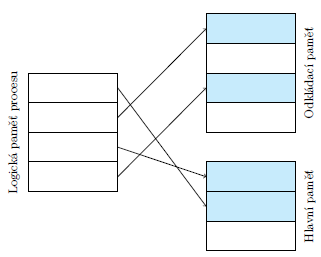
\includegraphics[scale=1]{images/mem_lap.png} \label{mem:lap}
\end{center}

Pokud počítač pracuje s 32bitovými adresami, může nabízet 4 GiB ($2^{32}$) LAP i když fyzicky má pouze 256 MiB FAP. Virtuální paměť lze realizovat mnoha způsoby:
\begin{itemize}
    \item Vyměňováním celých procesů
    \item Stránkováním
    \item Segmentací
\end{itemize}

\begin{Large}
    \vspace{0,5cm}
    \textbf{Vymeňování procesů}
\end{Large}

Jak již bylo zmíněno dřív, paměť lze přidělovat celým procesům nebo jejich částem. Ty jsou poté vyměňovány mezi hlavní a odkládací pamětí, tak aby se postupně vyměnili všechny procesy. Při práci s celými procesy se načte celý proces do paměti a po nějaké době je odložen do odkládací paměti (\textit{připraven v odkládací paměti}). Po určité době je vybrán plánovačem II. úrovně k přesunutí do hlavní paměti kde bude opět vybrán plánovačem I. úrovně k vykonání. 

\vspace{0,5cm}

Velikost a umístění využitých paměťových úseků se dynamicky mění podle toho který proces je načten do paměti (jaká je aktuální velikost jejich paměťového prostoru). Toto však způsobuje tzv. \textit{externí fragmentaci paměti} kdy vznikají v paměti volné úseky paměti, které však nejsou dostatečné velké pro kterýkoliv proces (nedochází pak k efektivnímu využívání paměti! viz obrázek níže s procesy A,B,C). Tento jev lze sice napravit tzv. \textit{defragmentací}, tedy spojením volných paměťových úseků a vytvoření souvislého paměťového prostoru.

\newpage

Aby se mohl tento úsek vytvořit je třeba přesunout všechny procesy do jednoho souvislého bloku zabrané paměti, tento proces je časově náročný (navíc by se musel dělat periodicky), proto se k němu většinou nepřikračuje. 

\begin{center}
    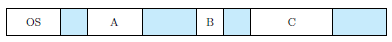
\includegraphics[scale=1]{images/mem_fragmentace.png}
\end{center}

Lze však proces rozdělit mezi hlavní a odkládací paměť díky jeho rozdělení na dílčí části (\textit{overlays}). Proces lze vykonávat pokud má v paměti svou první část, po dokončení se načte druhá apod. Nebo držet v paměti více částí procesu najednou. (viz Obrázek \ref{mem:lap})

\begin{Large}
    \vspace{0,5cm}
    \textbf{Stránkování}
\end{Large}

Paměťový prostor procesu je rozdělen na stejně velké části tzv. \textit{stránky} (\textit{pages}), které jsou v případě potřeby přesouvány z odkládací paměti do stejně velkých míst v hlavní paměti tzv. \textit{rámců} (\textit{frames}). Přenesení stránek do hlavní paměti je zavolání tzv. \textit{page fault} (\textit{výpadek stránky}), tedy že proces potřebuje pracovat se stránkou která právě v paměti není. Proces sám však \textit{page fault} nevyvolá, procesor rozpozná, že chybí stránka a zavolá \textit{výpadek}\footnote{Proces tuto výměnu ani nevidí, viditelný je pro OS, který vede evidenci jednotlivých stránek.}. Umístění stránek je uloženo v \textit{tabulce stránek} (page table).

\begin{center}
    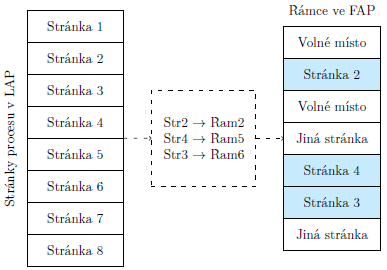
\includegraphics[scale=1]{images/mem_page_table.png}
\end{center}

Díky pevné velikosti stránek je lze efektivně umístit do stejně velkých rámců. Díky tomu nedochází k \textit{externí fragmentaci} volného prostoru v hlavní paměti. Nevýhodou je, že proces do této struktury nevidí, tudíž neví, že části které patří k sobě by se měli přesouvat do paměti společně za účelem zredukování množství \textit{page fault}.

\vspace{0,5cm}

Důležitým parametrem je volba velikosti stránky. Jelikož se stránkováním nemůže docházet k externí fragmentaci, ale k interní ano. Pokud jsou stránky moc velké, tak poslední stránka nebude nikdy kompletně naplněna a zůstane v ní nevyužitý prostor. Zároveň pokud proces vyžaduje 4 KiB paměti, ale stránky jsou 32 KiB, je potřeba do paměti načíst zbytečně 32 KiB. Zřejmě je asi výhodnější mít menší stránky. Na druhou stranu to však znamená větší počet výpadků stránek a větší tabulku stránek\footnote{Čas přenesení stránky je tvořen převážně jejím vyhledáním, proto doba přenosu malých stránek trvá přibližně stejně jako velkých.}. 

\newpage

\begin{Large}
    \vspace{0,5cm}
    \textbf{Segmentace}
\end{Large}

Pomocí segmentace je paměťový prostor procesů dělen na logicky související části různé velikosti nazývané \textit{segmenty}. Každý segment má svůj název a velikost, které vytváří kompilátor podle zdrojového kódu programu. Obecné segmenty mohou být:

\begin{itemize}
    \item Textový - instrukce programu.
    \item Datový - inicializované globální a statické proměnné.
    \item BSS (Block Started by Symbol) - neinicializované globální a statické proměnné, kde hodnota může být náhodná hodnota z paměti nebo O (pro ukazatele \textit{null}).
    \item Halda - dynamické proměnné.
    \item Zásobník
\end{itemize}

Blíže mohou být segmenty děleny například na:

\begin{itemize}
    \item Kódy jednotlivých funkcí
    \item Velké datové struktury
    \item Knihovny linkované s programem 
    \item Objekty
\end{itemize}

Na rozdíl od stránkování je segmentace mechanismus který je procesu viditelný. Pokud proces potřebuje nějakou část segmentu v hlavní paměti, tak je přenesen celý segment. Výhoda tohoto přístupu je, že jakmile je v dalších krocích potřeba další část segmentu nemusí být opět načten do paměti. Tímto je redukován počet výpadků segmentů (\textit{segment fault}) oproti výpadkům stránek. A stejně tak jako se stránkami vede operační systém záznamy o všech segmentech v tabulce segmentů (\textit{segment table}). 

\begin{center}
    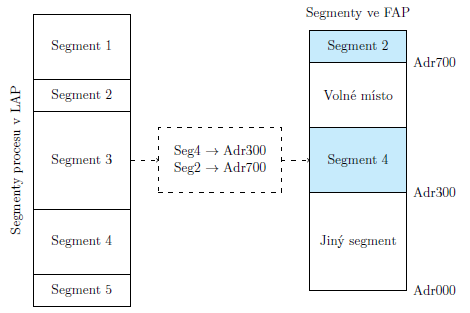
\includegraphics[scale=1]{images/mem_segment_table.png} \label{mem:segment-table}
\end{center}

Nevýhodou oproti stránkování je právě dynamická velikost segmentů, což způsobuje externí fragmentaci paměti (viz Obrázek výše).

%%%%%%%%%%%%%%%%%%
% VYUŽITÍ PAMĚTI %
%%%%%%%%%%%%%%%%%%

\newpage
\section{Využití paměti\,--\,přidělování paměti procesům, algoritmy přesunu stránek do odkládacího prostoru}

Existují tři základní způsoby přidělování hlavní paměti:
\begin{itemize}
    \item rovnoměrně - nerespektuje rozdílné paměťové nároky procesů a ani jejich prioritu
    \item podle velikosti procesu - nerespektuje prioritu procesu
    \item podle velikosti a priority procesu
\end{itemize}

Abychom mohli určit jaký počet rámců procesům přidělit, využíváme metodu na vyhodnocování frekvence výpadků stránek. Účelem je vyhnout se stavu, kdy je proces zdržován velkým množstvím výpadků stránek, tzv. \textit{trashing}. Proto se snažíme udržet frekvenci výpadků stránek na přibližně stejné úrovni, zároveň pokud dochází k příliš mnoha výpadkm značí to nedostatek rámců, a naopak pokud je výpadků moc málu má proces příliš mnoho paměti. Jedná se o tzv. algoritmus \textit{Page Fault Frequency Replacement}. 

\begin{center}
    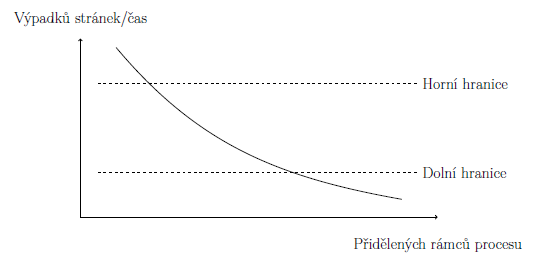
\includegraphics[scale=1]{images/mem_freq_page.png}
\end{center}

\begin{Large}
    \vspace{0,5cm}
    \textbf{Přesuny stránek}
\end{Large}

Jak již bylo zmíněno, virtuální paměť je založena na odkládání stránek z hlavní paměti do odkládací (na disk). Když je zavolán výpadek stránky je třeba přesunout jednu stránku do volného rámce. Operační Systém zajišťuje aby vždy byly dostupné volné rámce, proto periodicky přesunuje určitý počet stránek do odkládací paměti. 

\begin{large}
    \vspace{0,5cm}
    \textbf{Odkládací paměť}
\end{large}

Při odložení z hlavní paměti mohou nastat dvě situace podle dat ve stránce:

\begin{enumerate}
    \item Data jsou pouze pro čtení/nebyly provedeny změny - stránka je z hlavní paměti smazána
    \item Data byla změněna - stránka musí být přesunuta do virtuální paměti
\end{enumerate}

Stránky mohou být svázány s určitým souborem v sytému, takový soubor může obsahovat kód procesu (read-only data) nebo se jedná o soubor připojený do uživatelského kontextu procesu, tzv. \textit{paměťově mapovaný soubor}\footnote{Tyto soubory v paměti mohou být jak v režimu pouze pro čtení tak i pro zápis.}. Takto lze jednoduše sdílet soubor mezi procesy. Pro práci s tímto souborem se používají paměťové funkce, což zvyšuje rychlost operací čtení a zápisu. Nevýhodou může potencionální plýtvání paměti\footnote{Uvažujme stránky o velikosti 4KiB a soubor o velikosti 6KiB, pak musíme využít dvě stránky ale z toho jsou 2KiB nevyužity.}. 

\begin{center}
    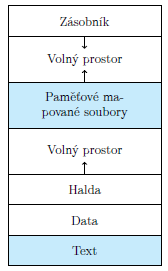
\includegraphics[scale=1]{images/mem_page_file.png}
\end{center}

\textit{Anonymní stránky} jsou stránky co nejsou svázané se souborem a jsou odkládány do speciálního \textit{odkládacího souboru} (\textit{swap file}) na \textit{odkládacím oddílu} (\textit{swap partition}) souborového systému. Jedná se o data z haldy a zásobníku.

\begin{center}
    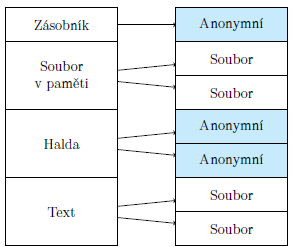
\includegraphics[scale=1]{images/mem_page_anon.png}
\end{center}

\begin{Large}
    \vspace{0,5cm}
    \textbf{Algoritmus LRU (Least Recently Used)}
\end{Large}

Funguje na předpokladu, že nedávno používané stránky budou patrně použity znovu a ty starší pravděpodobně ne. Z tohoto důvodu je třeba udržovat pořadový seznam všech stránek v hlavní paměti podle jejich doby použití. Na začátku je naposledy použitá stránka a na konci nejdéle nepoužitá. Seznam se navíc aktualizuje při každém použití stránky. Pro rychlé provedení algoritmu se využívá hardware.

\vspace{0,5cm}

Jedna z možností je použití hardware s 64 bitovým čítačem, který je inkrementován po vykonání každé instrukce. Každá stránka má přiděleno jedno návěští kde je hodnota čítače. Po použití stránky se do návěští uloží aktuální hodnota čítače. Když je potřeba odstranit stránku je vybrána ta s nejnižší hodnotou čítače, jelikož byla nižší hodnota čítače znamená, že již proběhlo mnoho instrukcí $\xrightarrow[]{}$ stará stránka. 

\newpage

Druhá možnost spočívá ve využití matic (opět v hardwaru). Pro \textit{n} možných stránek ve FAP je použita matice $n \times n$ bitů. Při každém použití stránky \textit{k} se nastaví bity řádku \textit{k} na 1 a poté se vynuluje sloupec \textit{k}. Řádek s nejnižší binární hodnotu patří stránce nejdéle nepoužité a je tedy vybrán\footnote{Skripta na straně 72 mají pěkný příklad}. 

\begin{Large}
    \vspace{0,5cm}
    \textbf{Algoritmus NFU (Not Frequently Used)}
\end{Large}

NFU je naopak softwarové řešení, které také využívá čítače. Pro každou stránku je udržován bit A (accessed), který je nastaven kdykoliv je daná stránka použita. Toto je monitorováno v intervalech daných přerušením od hodin, každý interval jsou všechny stránky prohledány a hodnota bitu A je přidána k čítači.  0 se přidává pokud ke stránce nebylo přistoupeno, 1 pokud bylo. Algoritmus vybírá stránku s nejnižší hodnotou čítače (stránka není často používaná). 

\vspace{0,5cm}

Nevýhodou klasického NFU je, že nikdy nenuluje hodnoty, preferuje tedy dříve často využívané stránky. Modifikovaný algoritmus tento problém \textit{stárnutí stránek} řeší následovně. Před přičtením hodnoty bitu A k čítači provede bitový posun o 1bit do prava (prakticky dělení dvěma). Následně je bit A přičten k bitu s nejvyšší váhou MSB (\textit{Most Significant Bit})\footnote{Prakticky bit co nejvíce vlevo.}. U klasického NFU to byl LSB (\textit{Least Significant Bit}). 

\vspace{0,5cm}

Nedostatky této modifikace:

\begin{itemize}
    \item Pokud má dojít k rozhodnutí mezi dvěma stránkami, vždy se vybere ta stránka s menší hodnotou čítače. Nemáme však záruku že se jedná o nejdéle nepoužitou stránku. 
    \item Čítače mají omezený počet bitů, po určitém čase mohou být všechny bity vynulované, pak nelze říct jestli byla stránka využita před \textit{n+1} intervaly (kde n je počet bitů čítače) nebo před 100 intervaly. Stránky jsou pak vybrány náhodně. 
\end{itemize} 

%%%%%%%%%%%%%%%%%%%%%
% SOUBOROVÉ SYSTÉMY %
%%%%%%%%%%%%%%%%%%%%%

\newpage
\section{Souborové systémy\,--\,organizace dat na paměťovém úložišti, metody ukládání datových bloků}

Souborový systém definuje jak jsou organizovaná data uložena na paměťovém médiu, a to jak vestavěném tak externím. Data jsou organizována ve formě souborů, které se potom sdružovány do adresářů\footnote{Adresářová struktura bývá poskádána hierarchicky. Pro jednouživatelské systémy se užívá \textit{plochý} systém, kde je jeden adresář a v něm všechny soubory.}. 

\vspace{0,5cm}

Souborové systémy udržují informace o umístění dat jednotlivých souborů na paměťovém médiu. Mimo to mohou poskytovat i časové informace (vytvoření a modifikace souboru). Ve víceuživatelských systémech se uchovávají i informace o \textit{vlastnících} a \textit{přístupových právech} k souboru. Informace o souboru dělíme na data a metadata:
\begin{itemize}
    \item data - obsah souboru.
    \item metadata - data potřebná pro práci se soubory jako informace o umístění, časová informace nebo přístupová práva. 
\end{itemize}

Paměťová média se typicky rozdělují na několik samostatných částí. První je \textit{MBR} (\textit{Master Boot Record}) obsahující zavaděč operačního systému, identifikátor disku a tabulku oddílů (\textit{partition table}) a může obsahovat i další části. MBR zavaděč je spouštěn kódem v BIOS (\textit{Basic Input-Output System}). Úkolem zavaděče je načíst zaváděcí sektor z aktivního oddílu, ten obsahuje Operační Systém který se spustí\footnote{Zaváděcí sektor se liší podle OS}. 

\begin{center}
    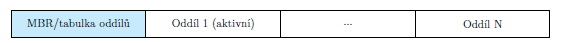
\includegraphics[scale=1]{images/mem_partitions.png}
\end{center}

V tabulce oddílů jsou uloženy informace o umístění jednotlivých oddílů, tedy kde začínají a kde končí. Na oddílech se mohou vyskytovat různé souborové systémy a na těch pak OS.

\begin{Large}
    \vspace{0,5cm}
    \textbf{Datové bloky}
\end{Large}

Souborové systémy ukládají soubory do tzv. \textit{datových bloků} (\textit{fragmentů}). Důležité je jak velký jeden blok je, jelikož velké bloky mohou podléhat \textit{interní fragmentaci} z důvodu, že je soubor nenaplní a \textit{datový blok} je nejmenší jednotka souborového systému. Naopak velmi malé bloky zpomalují operace se soubory, jelikož každý blok vyžaduje vyhledání jeho umístění. 

\begin{large}
    \vspace{0,5cm}
    \textbf{Kontinuální ukládání bloků}
\end{large}

Bloky jsou ukládány na paměťovém médiu za sebou, tento způsob je vhodný u plotnových disků, jelikož minimalizuje přesun čtecích hlav (mimo přesun hlav mezi cylindry). Záznam adresářů udržuje jen počáteční adresu souboru a počet bloků (tj. jeho velikost). Problém vzniká při rozšiřování souborů nebo zmenšování souborů. 

\vspace{0,5cm}

Navíc dochází k \textit{externí fragmentaci} skrz změny ve velikostech souborů vznikají volné oblasti mezi záznamy, 
které však nejsou dostatečně velké pro jakýkoliv soubor. 

\newpage

Procesu odstranění tohoto problému se říká \textit{defragmentace}, dělávalo se tak, že se přesunuly všechny využité bloky na jiné file systém, původní data (na původním oddílu) byla smazána. Nakonec byla data překopírována zpět v kontinuálním způsobu. Velmi časově náročné a muselo se vykonávat periodicky! 

\begin{large}
    \vspace{0,5cm}
    \textbf{Ukládání bloků nesouvisle s ukazateli v bloku}
\end{large}

Bloky nejsou na médiu rozděleny souvisle, místo toho je část jejich prostoru obětován ukazateli na další blok souboru. Při vytvoření souboru je nalezen volný blok kdekoliv na paměťovém médiu a je použit pro nová data\footnote{Pokud má soubor nulovou velikost je ukazatel nastaven jako neplatný.}. Takto prakticky funguje jako \textit{linked list} a nenastává problém s externí fragmentací. 

\vspace{0,5cm}

Avšak přesně tento přístup je nevýhodou této možnosti. Při čtení je potřeba nejprve načíst první blok a postupně hledat bloky pomocí ukazatelů. Každé načtení je tedy z jiného sektoru disku a zpomaluje program. Další problém je, že ukazatel ubírá místo z bloku. Řešením pro tento problém je seskupit bloky a zavést ukazatel na ně, pointer pak zabírá menší procenty paměti a urychluje se práce s daty. Bohužel ale dochází k \textit{interní fragmentaci}\footnote{Existuje i možnost poškození ukazatele, pokud se jedná o první ukazatel tak se přijde o celý soubor.}.

\begin{large}
    \vspace{0,5cm}
    \textbf{Ukládání bloků nesouvisle s ukazateli v indexačním bloku}
\end{large}

Funguje prakticky stejně jako předešlá implementace, akorát ukazatele nejsou obsaženy v samotném bloku, nýbrž v tabulce ukazatelů pro daný soubor (udržováno ukazatelem v adresáři kde se soubor vyskytuje). Při vytvoření jsou všechny ukazatele neplatné, při zápisu dat do volných bloků se postupně aktualizují ukazatele. 

\vspace{0,5cm}

Nedochází sice k externí fragmentaci, ale k plýtvání paměti. Pokud se vytvoří malý soubor tak bude zabrán jeden celý blok navíc pro udržování indexační tabulky, který se však nezaplní. Proto je třeba vhodně volit velikost tabulky.

\vspace{0,5cm}

Přístupy pro práci s indexačními bloky:
\begin{itemize}
    \item Přímé odkazy - indexační blok obsahuje ukazatele na datové bloky, v případě velkého souboru lze propojit více indexačních bloků, poslední ukazatel je tedy buď neplatný (pro malé soubory) nebo ukazuje na začátek další tabulky.
    \item Nepřímé odkazy - indexační blok obsahuje odkazy na další indexační bloky, které obsahují přímé odkazy na datové bloky. Pro přístup k blokům se nejprve načte indexační blok přes nepřímý odkaz a až poté se načte blok přes přímý odkaz. 
    \item Kombinace - Indexační blok obsahuje přímé i nepřímé a dokonce i zanořené nepřímé odkazy, tedy nepřímý odkaz na nepřímý odkaz. Je vhodný pro velké soubory (nepřímé odkazy s několika úrovněmi) i pro malé soubory (přímé odkazy).
\end{itemize}

\begin{center}
    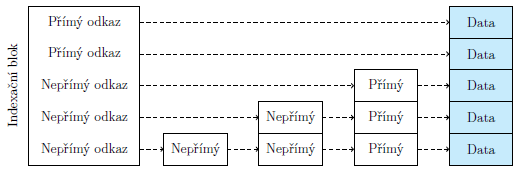
\includegraphics[scale=1.2]{images/mem_block_index.png}
\end{center}

\begin{Large}
    \vspace{0,5cm}
    \textbf{Ukládání dat a metadat na HDD}
\end{Large}

Pevný disk se skládá z ploten\footnote{Pro čtení z ploten se používá více hlav.} (které jsou uspořádány nad sebou), které jsou rozděleny na stopy a ty zase na sektory. Sektor je nejmenší jednotka pro ukládání dat na pevném disku. Datové bloky souborových systémů, mohou zabírat jeden nebo více sektorů. Při práci s daty se nejprve načtou metadata o souboru (přístupová práva a o uložení dat), tedy hlavice musí přejít na pozici metadat a až poté na pozici dat\footnote{Přilíž velkému množství přesunů se zamezuje pomocí organizace do tzv. \textit{cylindrů}, což je sada nad sebou umístěných stop. Tyto společně udržují data a metadata.}.  

\begin{center}
    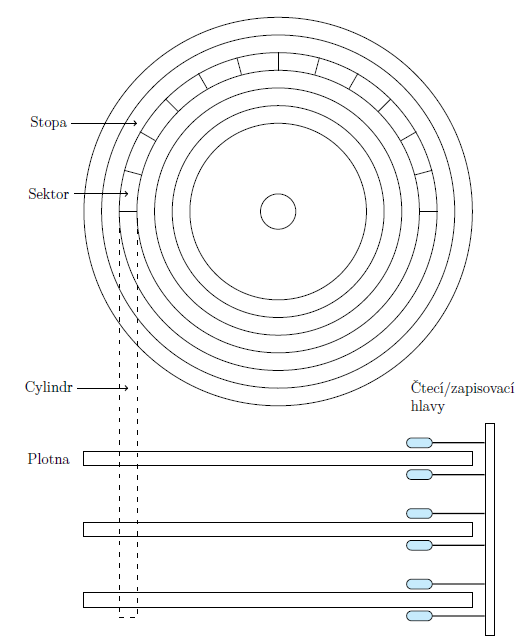
\includegraphics[scale=1]{images/mem_hdd.png}
\end{center}

%%%%%%%%%%%%%%%
% KONZISTENCE %
%%%%%%%%%%%%%%%

\newpage
\section{Konzistence dat\,--\,data a metadata, žurnálovací souborové systémy}

Když se v souborovém systému pracuje s daty (zapisování a mazání), může dojít k situaci kdy se data dostanou do nekonzistentního stavu, z důvodu pádu systému. Nekonzistentními situacemi mohou být:

\begin{itemize}
    \item Soubor nebyl smazán, i když k tomu byl zadá požadavek.
    \item Část dat byla aktualizována zápisem, další část ne. 
\end{itemize}

Jak probíhá mazání souboru?

\begin{enumerate}
    \item Odstranění záznamu o souboru z adresáře,
    \item uložení čísla i-uzlu (viz dále) souboru do seznamu volných i-uzlů,
    \item uložení datových bloků souboru do seznamu volných bloků k použití.
\end{enumerate}

Pokud dojde k pádu systému mezi kroky 1 a 2, tak zůstane i-uzel v použitém stavu i když tomu tak není. Tato skutečnost plýtvá pamětí, jelikož i-uzel nemůže být využit pro jiná data. Podobná situace nastává při pádu mezi kroky 2 a 3. Jako řešení tohoto problému byly navrhnuty žurnálovací systémy (také viz dále). 

\begin{Large}
    \vspace{0,5cm}
    \textbf{Ukládání metadat}
\end{Large}

Metadata se ukládají ve speciální struktuře, zvané \textit{i-uzel}\footnote{Detaily budou specifické pro OS Linux} (tj. \textit{i-node}). Tyto struktury obsahují metadata o souboru, jako typ souboru, vlastník, skupina vlastníka, přístupová práva, délka souboru, čas vytvoření, čas posledního přístupu a čas modifikace. Dále i-uzel obsahuje ukazatele na bloky souboru. 

\vspace{0,5cm}

V adresářích se vyskytují položky obsahující jméno souboru a číslo relevantního \textit{i-uzlu}, tyto informace jsou důležité pro nalezení souborů. Navíc může být v různých adresářích více souborů se stejným jménem ukazující na jeden soubor/\textit{i-uzel} (tj. \textit{pevné odkazy}/\textit{hard link})\footnote{Při smazání pevného odkazu je počet těchto odkazů snížen o jedno. Pokud je počet roven 0 je soubor definitivně smazán.}.

\vspace{0,5cm}

Dále existuje \textit{symbolický odkaz} (\textit{symlink}), kdy soubor odkazuje na jiný. Při smazání souboru, na který \textit{symlink} odkazuje, nedochází ke smazání souboru se symbolickým odkazem. 

\newpage

\begin{Large}
    \textbf{Žurnálovací souborové systémy}
\end{Large}

Tyto systémy udržují ve svém $"$žurnálu$"$ záznamy o plánovaných změnách před jejich provedením. Pokud dojde k pádu systému, je schopen dostat data a metadata do konzistentního stavu pomocí předešle uložených plánů operací v žurnálu. 
Uložená operace je však proveditelná, pouze pokud je kompletně uložená. 

\vspace{0,5cm}

Pokud není operace zapsána jako celek do žurnálu před pádem systému, je ignorována. Kontrolu lze provádět pomocí kontrolního součtu, v případě pádu systému před kompletním zápisem do žurnálu nebude součet sedět a zápis bude ignorován.

\vspace{0,5cm}

Do žurnálu lze ukládat pouze metadata nebo metadata a vlastní data souboru. Je jasné, že první varianta je rychlejší ale s možností ztráty konzistence, zatímco druhá možnost je pravý opak.

\begin{itemize}
    \item Při ukládání pouze metadat může dojít k inkonzistenci mezi metadaty. Např. při přidání dat do souboru:
    \begin{enumerate}
        \item Změna záznamu o velikosti souboru v jeho i-uzlu (metadata).
        \item Z volných datových bloků je vybrán prostor pro nová data (metadata).
        \item Do vybraných bloků jsou zapsány data (data). 
    \end{enumerate}
    Pokud dojde k pádu systému před třetím krokem, budou v žurnálu zaznamenány datové bloky, ale v těch bude náhodná změť paměti. 
    
    \item Při ukládání s daty souborů jsou do žurnálu ukládány kopie všech datových bloků do kterých se bude zapisovat. Pokud dojde k pádu, je operace zápisu provedena znovu nad kopií datových bloků. Toto ,samo sebou, značně zpomaluje operaci zápisu. Využívá se pouze v systémech, kde vyžadujeme naprostou ochranu dat. 
\end{itemize}

Základní implementace:

\begin{enumerate}
    \item Kopie žurnálu mohou být umístěny na různých paměťových médiích za účelem zálohování v případě poruchy jiného média.
    \item Plánované změny v žurnálu mohou být dále ukládány v jiném žurnálu z důvodu zvýšení redundance.
    \item Žurnál je ukládán na stejném nebo jiném médiu, z důvodu vyšší rychlosti. 
\end{enumerate}

\newpage
\section{Síťová část OS\,--\,stavy soketů při komunikaci, síťová systémová volání, serverové procesy}
